% no answer key
\documentclass[letterpaper]{exam}

% answer key
% \documentclass[letterpaper, landscape]{exam}
% \usepackage{2in1, lscape} 
% \printanswers

\usepackage{units} 
\usepackage{graphicx}
\usepackage[fleqn]{amsmath}
\usepackage{cancel}
\usepackage{float}
\usepackage{mdwlist}
\usepackage{booktabs}
\usepackage{polynom}
\usepackage{caption}
\usepackage{fullpage}
\usepackage{comment}
\usepackage{enumerate}
\usepackage{parskip}
\usepackage{xfrac}

\newcommand{\degree}{\ensuremath{^\circ}} 
\everymath{\displaystyle}

% \printanswers
\excludecomment{comment}
\addpoints

\title{Math 142 \\ Chapter One Exam}
\date{\today}
\author{}

\begin{document}

  \maketitle

  \begin{center}
    \gradetable[h][pages]
  \end{center}

  \section{Questions}

  Figure \ref{fig:exams} is a scatter plot of midterm vs. final exam test scores
  for a class.

  Questions \ref{q:exams.first}-\ref{q:exams.last} refer to Figure \ref{fig:exams}.  

  \begin{figure}[H]
    \centering
    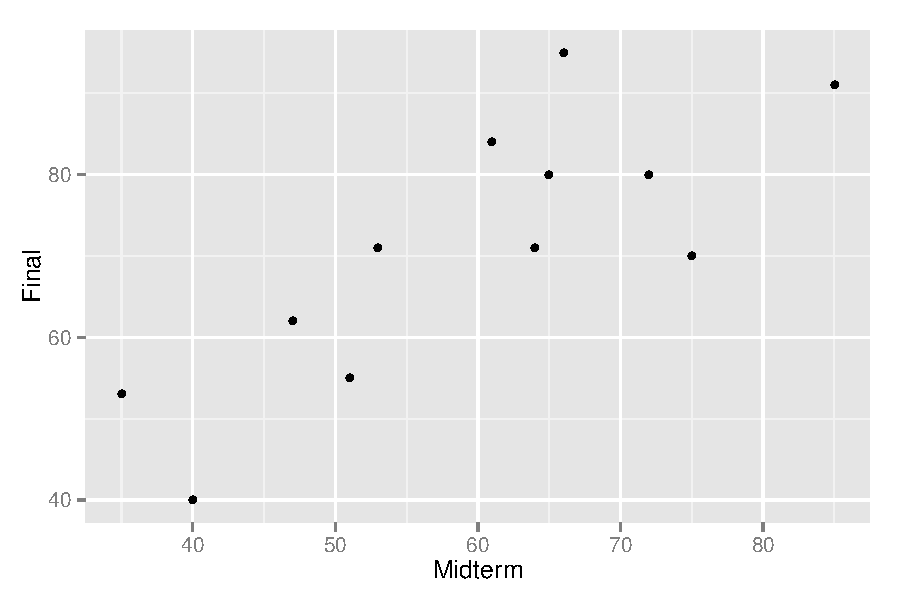
\includegraphics[scale = 0.5]{figures/exams_scatter.pdf}
    \caption{Questions \ref{q:exams.first}-\ref{q:exams.last}}
    \label{fig:exams}
  \end{figure}

  \begin{questions}
    
    % \question
    %   \[
    %      x = \{ 1, 5, 8, 12 \}
    %   \]

    %   \begin{parts}
    %     \part[2] What is $\bar{x}$.

    %       \begin{solution}
    %         $\bar{x} = 6.5$
    %       \end{solution}

    %     \part[3] What is the expression for $s_x$?
    %       \begin{solution}
    %         \[
    %           s_x = \sqrt{\frac{(1 - 6.5)^2 + (5 - 6.5)^2 + (8 - 6.5)^2 
    %             + (12 - 6.5)^2}{3}}
    %         \]
    %       \end{solution}

    %   \end{parts}


    \question[3] Estimate the mean score on the final for people who scored more than
      60 on the midterm:
      \label{q:exams.first}

      \begin{enumerate}[(a)]
        \item about 70
        \item about 80
        \item about 90
      \end{enumerate}

    \question[3] Estimate the correlation coefficient:
      \begin{enumerate}[(a)]
        \item about 0.5
        \item about 0.8
        \item about 0.99
      \end{enumerate}

    \question
      \label{q:exams.last}
      \begin{parts}
        
        \part[8] Draw box plots for the midterm and final
          \ifprintanswers
            \begin{figure}[H]
              \centering
              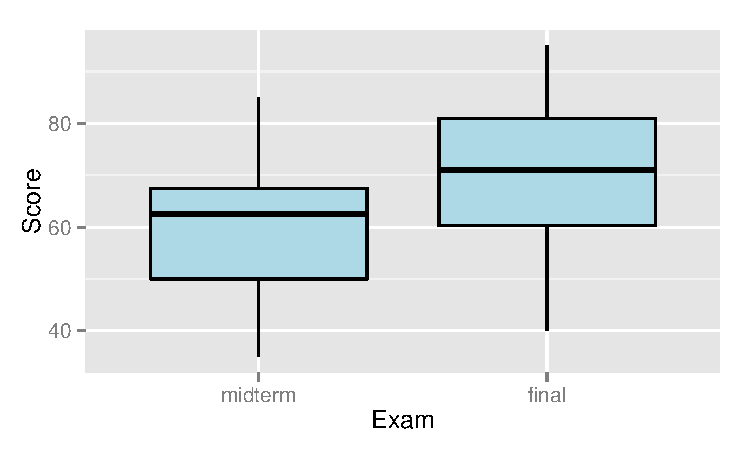
\includegraphics[scale = 0.8]{figures/exams_box.pdf}
              \caption{Question \ref{q:exams}}
              \label{fig:exams_box}
            \end{figure}
          \fi

        \part[2] Compared to the midterm, was the final exam 
          \begin{enumerate}[(a)]
            \item harder 
            \item easier
            \item about the same difficulty
          \end{enumerate}

      \end{parts}

    \question
      \label{q:point.histogram}
      Here are the average points per game for some NBA starting players:

      \begin{table}[ht]
        \centering
        \begin{tabular}{lr|lr}
          \toprule
          Player                   & Points & Player                 & Points\\
          \midrule
          Trey Burke               & 12.3   & LeBron James           & 27.2 \\
          Kentavious Caldwell-Pope & 6.0    & Michael Kidd-Gilchrist & 7.4 \\
          Tyson Chandler           & 9.3    & Robin Lopez            & 10.8 \\
          Glen Davis               & 12.1   & Kevin Martin           & 19.2 \\
          Jared Dudley             & 7.3    & Ben McLemore           & 7.6 \\
          Kevin Durant             & 31.8   & Chandler Parsons       & 16.6 \\
          Raymond Felton           & 10.0   & Kendrick Perkins       & 3.4 \\
          Randy Foye               & 12.6   & Zach Randolph          & 17.1 \\
          Marc Gasol               & 13.7   & Terrence Ross          & 10.7 \\
          Paul George              & 22.2   & Jared Sullinger        & 12.9 \\
          Spencer Hawes            & 13.0   & P.J. Tucker            & 9.3 \\
          Dwight Howard            & 18.9   & Evan Turner            & 16.6 \\
          \bottomrule
        \end{tabular}
      \end{table}

      \begin{parts}
        \part[10] Draw a histogram with a bin width of 5 points for these players.
        \ifprintanswers
          \begin{figure}[H]
            \centering
            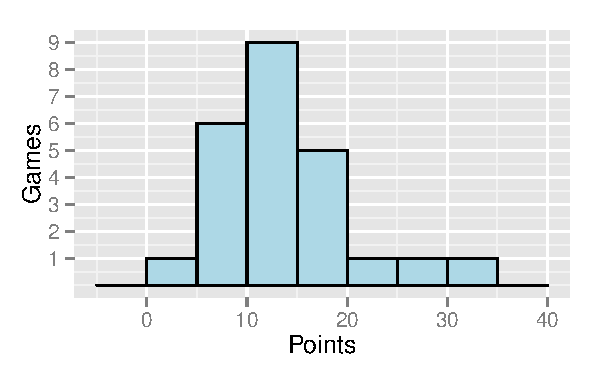
\includegraphics[scale = 1]{figures/point_histogram.pdf}
            \caption{Question \ref{q:point.histogram}}
            \label{fig:point.histogram}
          \end{figure}
        \fi

        \part[2] Is the distribution symmetrical, left-skewed, or right-skewed?
        \begin{solution}
          right-skewed
        \end{solution}

        \part[3] Is the mean higher or lower than the median?  Explain how you
          can know the answer without calculating the actual values.
          \begin{solution}
            Because the distribution is right-skewed, the mean while be larger than
            the median.
          \end{solution}

        \part[3] Is the median or mean a better measure of the center of this
          distribution?  Why?

          \begin{solution}
            Since this is a skewed asymmetrical distribution, the median is a better
            measure of the center.  The median indicates what a typical player is
            likely to score, while the mean is heavily influenced by a few high
            scoring players.
          \end{solution}

      \end{parts}

    \question
      There is heated debate this year about whether Kevin Durant or
      LeBron James should be the MVP.  

      Here is a representative selection of the number of points they scored in
      selected games this season:

      \begin{tabular}[H]{ll}
        Durant & \{ 13, 17, 19, 24, 26, 28, 29, 31, 32, 32, 32, 37, 41, 42, 42 \} \\
        James  & \{ 13, 15, 17, 19, 25, 25, 25, 26, 29, 30, 32, 33, 35, 36, 36 \} \\ 
      \end{tabular}

      \begin{parts}
        \part[8] Find the 5-number summary for both players
        \part[6] Draw a box plot for both players
        \part[3] Which player seems to be the MVP, based solely on points scored in
        these games? 
      \end{parts}

    % \question
    %   The MVP award is about how much you help your team, particularly in close
    %   games.  Tables \ref{tab:durant_diff} and \ref{tab:james_diff} show the points
    %   scored by each player in games which were decided by less than 5 points.  The
    %   ``Final Score'' is the difference between the Durant/James team and the score
    %   of whoever they were playing.

    %   The correlation coefficients and standard deviations are:

    %   \begin{table}[ht]
    %     \centering
    %     \begin{tabular}{rr}
    %       \toprule
    %       Points & Final Score \\
    %       \midrule
    %       42     & 3 \\
    %       33     & 1 \\
    %       20     & -1 \\
    %       38     & 2 \\
    %       25     & 1 \\
    %       27     & 2 \\
    %       28     & 3 \\
    %       34     & 4 \\
    %       37     & -4 \\
    %       24     & -2 \\
    %       48     & 4 \\
    %       37     & -3 \\
    %       41     & 2 \\
    %       29     & -1 \\
    %       36     & 3 \\
    %       43     & 4 \\
    %       \bottomrule
    %     \end{tabular}
    %     \caption{Durant points and final score differential}
    %     \label{tab:durant_pt_diff}
    %   \end{table}

    %   \begin{table}[ht]
    %     \centering
    %     \begin{tabular}{rrr}
    %       \toprule
    %       Points & Final Score \\
    %       \midrule
    %       25     & -1 \\
    %       22     & -3 \\
    %       31     & 4 \\
    %       26     & 3 \\
    %       24     & 3 \\
    %       36     & 1 \\
    %       26     & 1 \\
    %       38     & 2 \\
    %       25     & -4 \\
    %       22     & 2 \\
    %       \bottomrule
    %     \end{tabular}
    %     \caption{James points and final score differential}
    %     \label{tab:james_pt_diff}
    %   \end{table}

    %   \begin{parts}
    %     \part[10] Make a scatter plot for each player using points as the explanatory
    %       variable and point differential as the response variable.

    %     \part[10] Find the equation for the regression line for each player and add
    %     regression lines to the two scatter plots.

    %     \part[3] If LeBron scores 30 points in a close game, what would you expect
    %     his team's margin of victory to be?

    %     \part[2] How confident can you be in the accuracy of the prediction from part c?

    %     \part[3] Based on this analysis, which player deservers the MVP award?
    %   \end{parts}

    %   \question
    %     Tables \ref{tab:durant_pt_diff} and \ref{tab:james_pt_diff} can also be used
    %     to predict how many points the two players would need to score in order to
    %     win a close game.

    %     \begin{parts}
    %       \part[5]
    %         Find the equation for the regression line for Kevin Durant with the final
    %         score as the explanatory variable and Durant's parts as the response
    %         variable.

    %       \part[5] Use the regression line to determine about how many points Durant would
    %       need to score in order for his team to win a close game by 2 points.

    %       \part[2] How confident can you be in the accuracy of the prediction from 
    %         part b?
    %     \end{parts}
        
      \question
        Three point shooting accuracy in 2013 is a roughly Normal distribution with a
        mean of 0.36 and a standard deviation of 0.05.

        \begin{parts}
          \part[5] Carmelo Anthony's three point shooting accuracy is 0.42 this
          year.  What is the z-score for this value?

          \begin{solution}
            \[
              \frac{0.42 - 0.36}{0.05} \approx \boxed{ 1.2 }
            \]
          \end{solution}

          \part[5] What percentage of the three point shooters in the NBA are less
            accurate than Melo?
            \begin{solution}
              about 0.8849 or 88.5\%
            \end{solution}

          \part[5]
            What is the three shooting accuracy for someone who is better than 20\%
            of the three point shooters?

            \begin{solution}
              about 0.3179 
            \end{solution}

        \end{parts}
        
      \newpage

      \uplevel{
        Table \ref{tab:sbp} shows the shots made and missed by
            position for NBA players in the 2013-14 season.

        Use Table \ref{tab:sbp} to answer questions \ref{q:sbp.first}-\ref{q:sbp.last}.

        \begin{table}[H]
          \centering
          \begin{tabular}{lrr}
            \toprule
            position       & missed & made \\
            \midrule
            Center         & 11105  & 11372 \\
            Power Forward  & 18972  & 17601 \\
            Small Forward  & 19583  & 15090 \\
            Shooting Guard & 20721  & 15617 \\
            Point Guard    & 20791  & 15087 \\
            \bottomrule
          \end{tabular}
          \caption{Shots by position}
          \label{tab:sbp}
        \end{table}
      }

      \question[5] Make a bar chart showing shots made for each position.  Order
        the bars by number of shots made, with the most productive position first.
        \label{q:sbp.first}

      \question[5] Make a table showing the marginal distributions of shots made
      for each position.

      \question 
        \label{q:sbp.last}
        \begin{parts}
          \part[5] Make a table showing the conditional distributions of percentage
          of shots made and missed for each position.  

          \part[2] Which position seems to contain the most accurate shooters?  Do
          you think this is because they are the most skilled shooters or is there
          a lurking variable that explains the shooting percentage differences?
          
        \end{parts}
      
      \newpage

      \question
        \label{q:draft}

        \begin{figure}[H]
          \centering
          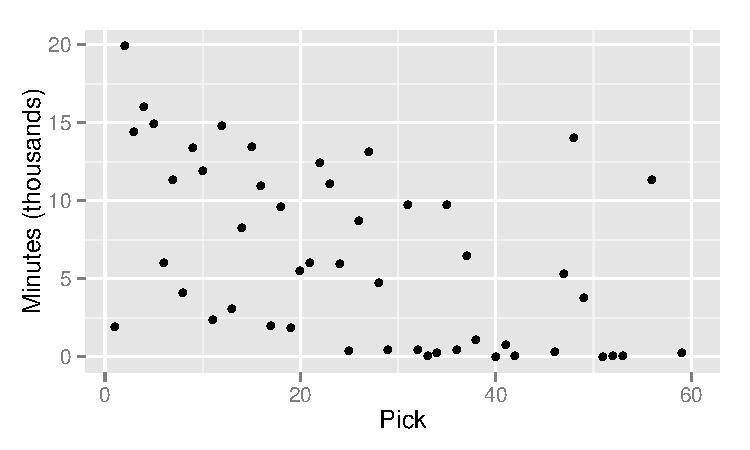
\includegraphics[scale = 1]{figures/draft.pdf}
          \caption{Question \ref{q:draft}}
          \label{fig:draft}
        \end{figure}

        \begin{table}[H]
          \centering
          \begin{tabular}{lrr}
            \toprule
                     & mean   & s \\
            \midrule
            Pick     & 30.5   & 17.5 \\
            Minutes  & 5218.9 & 5697.6 \\
            \bottomrule
          \end{tabular}
          \caption{Question \ref{q:draft}}
        \end{table}

        Figure \ref{fig:draft} shows the total number of minutes played vs.  draft
        order for the 2008 draft.  The better players are generally drafted first
        and also usually play more, so there is a negative correlation of 
        $r = -0.6020$ between draft order and minutes played.

        The first two selections in the 2008 draft were Greg Oden and Kevin Durant.
        As you can see in the chart, Greg Oden has had an injury plagued career and
        has only played 1940 minutes while Devin Durant has had a successful and so
        far mostly injury free career and has played nearly 20,000 minutes

      \begin{parts}
        \part[7]
          Find the equation for the regression line using the draft pick as the
          explanatory variable and minutes played as the response variable.

        \part[5] Graph the regression line.

        \part[2] What percentage of the variation in the minutes played is
        accounted for by the linear regression line?

        \part[3] Mark Gasol and Ramon Sessions are outliers because they were late
        round draft picks (pick 48 and 56) who have had a successful NBA careers
        with over 11,000 minutes each so far.

        Would removing these data points from the graph have a significant effect
        on the regression line?  Why or why not? 

      \end{parts}


  \end{questions}
\end{document}

